%%%%%%%%%%%%%%%%%%%%%%%%%%%%%%%%%%%%%%%%%
% University/School Laboratory Report
% LaTeX Template
% Version 3.1 (25/3/14)
%
% This template has been downloaded from:
% http://www.LaTeXTemplates.com
%
% Original author:
% Linux and Unix Users Group at Virginia Tech Wiki 
% (https://vtluug.org/wiki/Example_LaTeX_chem_lab_report)
%
% License:
% CC BY-NC-SA 3.0 (http://creativecommons.org/licenses/by-nc-sa/3.0/)
%
%%%%%%%%%%%%%%%%%%%%%%%%%%%%%%%%%%%%%%%%%

%----------------------------------------------------------------------------------------
%	PACKAGES AND DOCUMENT CONFIGURATIONS
%----------------------------------------------------------------------------------------

\documentclass[12pt]{article}

\usepackage[hmargin=3cm, vmargin=2cm]{geometry} % set margins

\usepackage{graphicx} % Required for the inclusion of images
\usepackage{natbib} % Required to change bibliography style to APA
%\usepackage{amsmath} % Required for some math elements 
\usepackage[utf8]{inputenc} % Use UTF-8
\usepackage{float}
\usepackage{booktabs}
\usepackage{listings}
\usepackage{amsmath}
\usepackage{color}

\definecolor{mygreen}{rgb}{0,0.6,0}
\definecolor{mygray}{rgb}{0.5,0.5,0.5}
\definecolor{mymauve}{rgb}{0.58,0,0.82}

\lstset{ %
  backgroundcolor=\color{white},   % choose the background color; you must add \usepackage{color} or \usepackage{xcolor}
  basicstyle=\footnotesize,        % the size of the fonts that are used for the code
  breakatwhitespace=false,         % sets if automatic breaks should only happen at whitespace
  breaklines=true,                 % sets automatic line breaking
  captionpos=b,                    % sets the caption-position to bottom
  commentstyle=\color{mygreen},    % comment style
  deletekeywords={...},            % if you want to delete keywords from the given language
  escapeinside={\%*}{*)},          % if you want to add LaTeX within your code
  extendedchars=true,              % lets you use non-ASCII characters; for 8-bits encodings only, does not work with UTF-8
  keepspaces=true,                 % keeps spaces in text, useful for keeping indentation of code (possibly needs columns=flexible)
  keywordstyle=\color{blue},       % keyword style
  language=Python,                 % the language of the code
  otherkeywords={*,...},           % if you want to add more keywords to the set
  numbers=none,                    % where to put the line-numbers; possible values are (none, left, right)
  numbersep=5pt,                   % how far the line-numbers are from the code
  numberstyle=\tiny\color{mygray}, % the style that is used for the line-numbers
  rulecolor=\color{black},         % if not set, the frame-color may be changed on line-breaks within not-black text (e.g. comments (green here))
  showspaces=false,                % show spaces everywhere adding particular underscores; it overrides 'showstringspaces'
  showstringspaces=false,          % underline spaces within strings only
  showtabs=false,                  % show tabs within strings adding particular underscores
  stepnumber=2,                    % the step between two line-numbers. If it's 1, each line will be numbered
  stringstyle=\color{mymauve},     % string literal style
  tabsize=2,	                   % sets default tabsize to 2 spaces
  title=\lstname                   % show the filename of files included with \lstinputlisting; also try caption instead of title
}

\setlength\parindent{0pt} % Removes all indentation from paragraphs

\graphicspath{{images/}} % Define graphics path

\renewcommand{\labelenumi}{\alph{enumi}.} % Make numbering in the enumerate environment by letter rather than number (e.g. section 6)

\renewcommand{\baselinestretch}{1.5} % set line spacing

\usepackage{times} % Uncomment to use the Times New Roman font

%----------------------------------------------------------------------------------------
%	DOCUMENT INFORMATION
%----------------------------------------------------------------------------------------

\title{Data Analysis and Knowledge Discovery \\ Exercise Work 2} % Title

\author{Tatu Seppä-Lassila} % Author name

\date{\today} % Date for the report

\begin{document}

\maketitle % Insert the title, author and date

%----------------------------------------------------------------------------------------
%	SECTIONS
%----------------------------------------------------------------------------------------
 
\section{Task 1: Wine Quality Prediction with Linear Regression}

In this task, scikit-learn's LinearRegression method was used. It takes two arguments: input variables and output variables. Therefore, input variables and output variable (quality) was separated from the data to their own variables. After that LinearRegression was called and model was fitted using fit method:

\begin{lstlisting}[language=Python]
lm = LinearRegression()
lm.fit(x,y)
\end{lstlisting}

After fitting, intercept and coefficients can be obtained and those can be combined to weight vector:

\begin{lstlisting}[language=Python]
# Get intercept and coefficients
coefs = lm.coef_
intercept = lm.intercept_
# Combine them to get the weight vector
weightVector = np.hstack((np.array(intercept), np.array(coefs)))
\end{lstlisting}

Result is the following weight vector presented here in two rows to save horizontal space:

\[
\begin{bmatrix}
 150.19284 & 0.06552 & -1.86318 & 0.02209 & 0.08148 & -0.24728 \\
 0.00373 & -0.00029 & -150.28418 & 0.68634 & 0.63148 & 0.19348
\end{bmatrix}
\]

I assume the method provides the best weight vector for the samples automatically.

\vspace{5mm} %5mm vertical space

After the initial setup, quality can be predicted with "predict" method. The method takes sample with input variables as its argument.

\vspace{5mm} %5mm vertical space

For calculating out-of-sample and in- sample error vectors, the data was splitted to five parts using numpy's "array\_split" method. In out-of-sample error calculation, each data part is iterated through and predicted quality is subtracted from actual quality. The result is added to the error vector of the data part. So in the end five error vectors are constructed.

For calculating in-sample error vectors, "combinations" method from Python's itertools was used to calculate combinations in which one data part is excluded from the rest of the five data parts. With five data parts, there are five combinations. After calculating combinations, four data parts in each combination was combined together. Finally, the abovementioned procedure was used to calculate error values and constructing error vectors.

The out-of-sample and in-sample error vectors were concatenated and error histograms were plotted using concatenated error vectors.

% Out-of-sample error histogram
\begin{figure}[H]
    \centering
    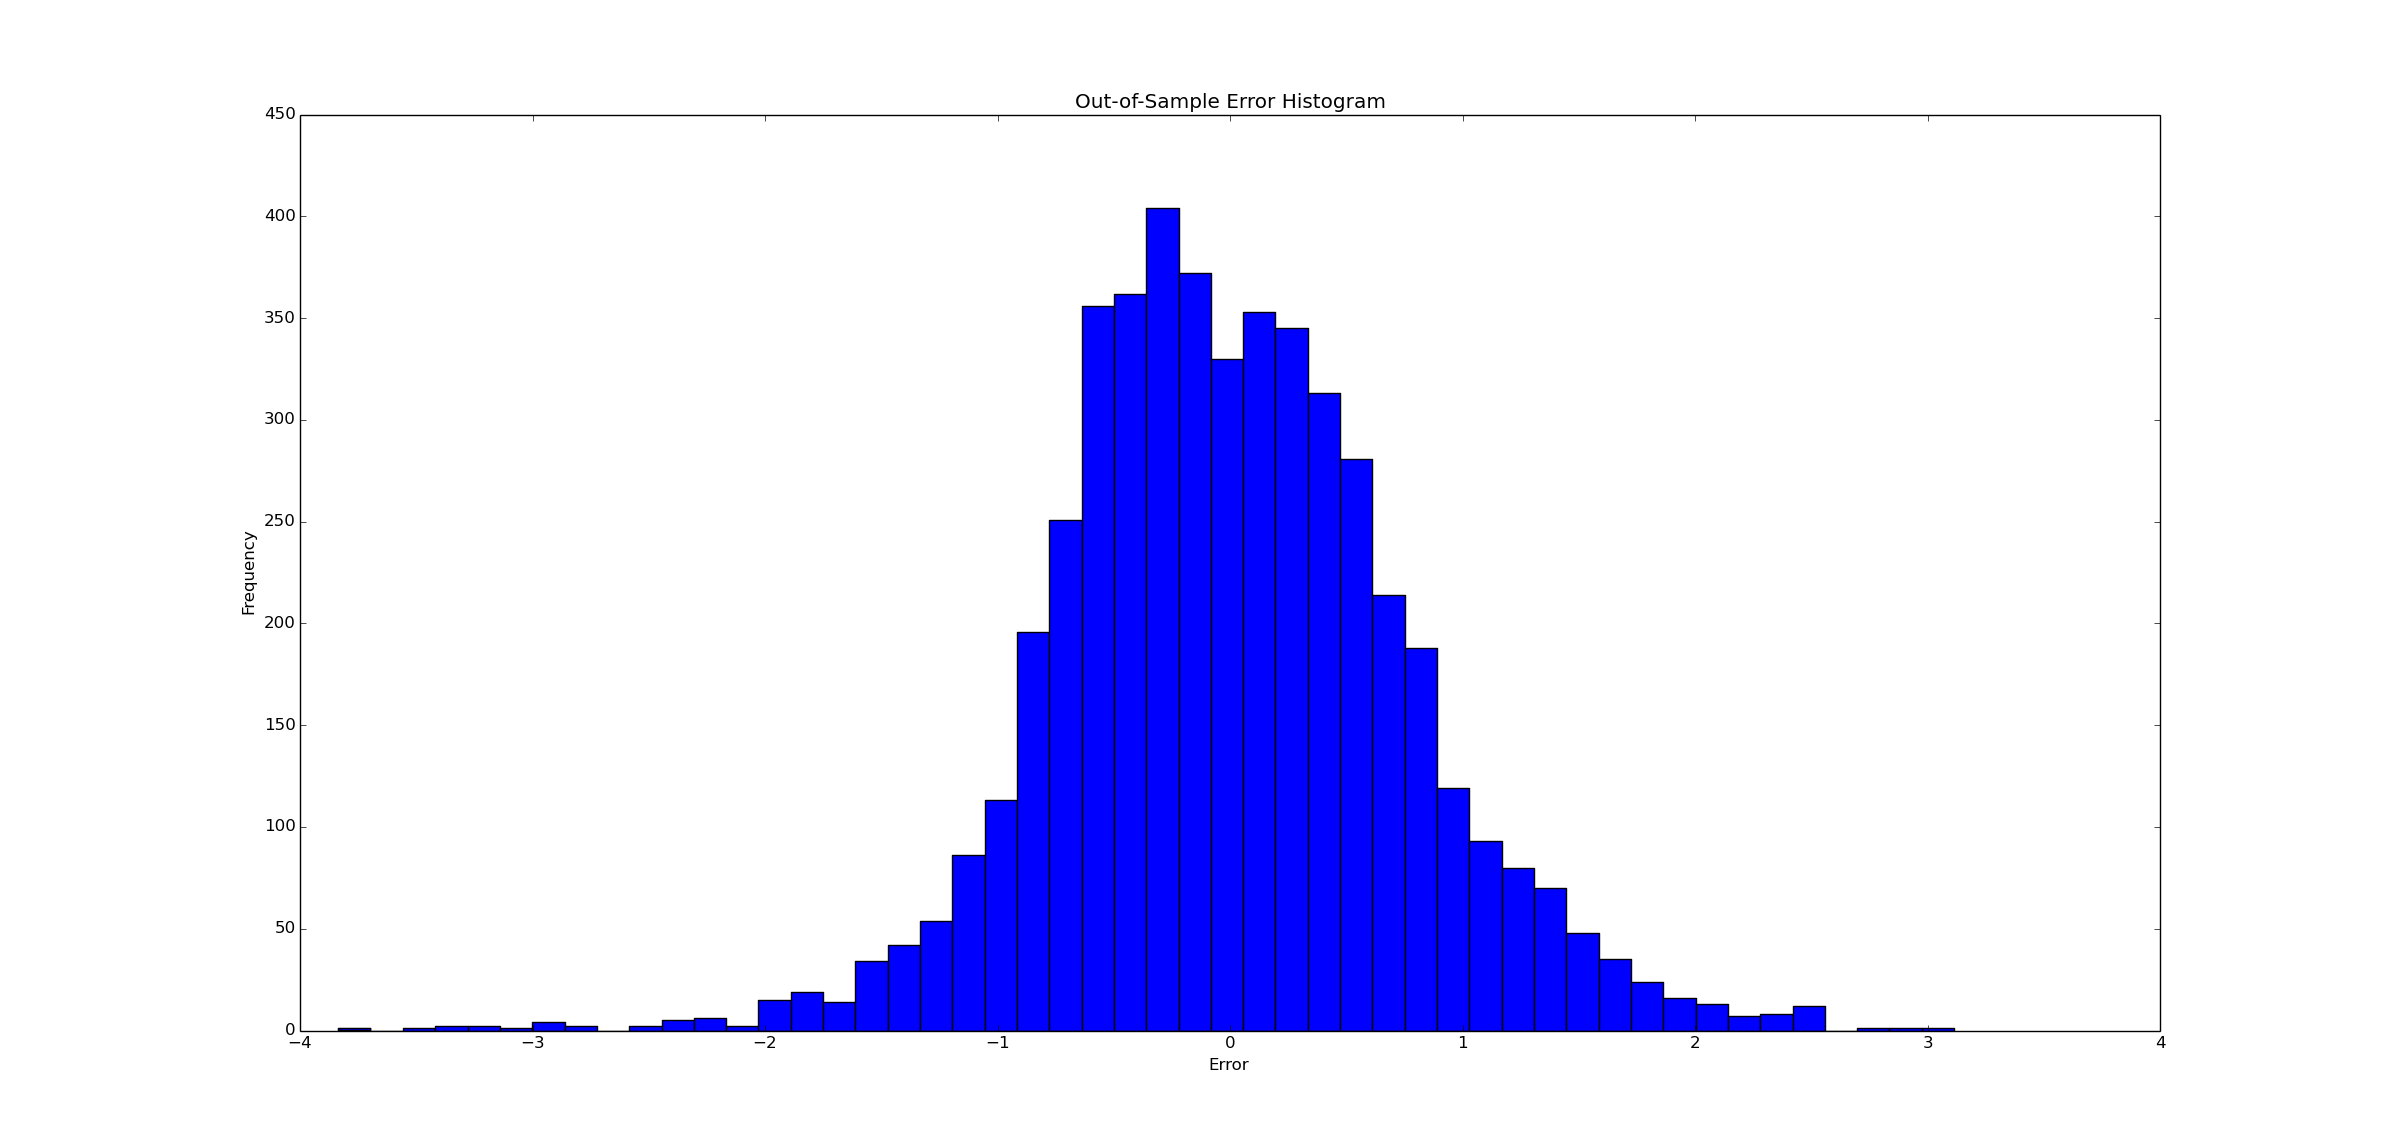
\includegraphics[width=1\textwidth]{figures/task1/oos_error_histogram}
    \caption{Out-of-sample error histogram plotted with matplotlib}
    \label{fig:oos_task1}
\end{figure}

% In-sample error histogram
\begin{figure}[H]
    \centering
    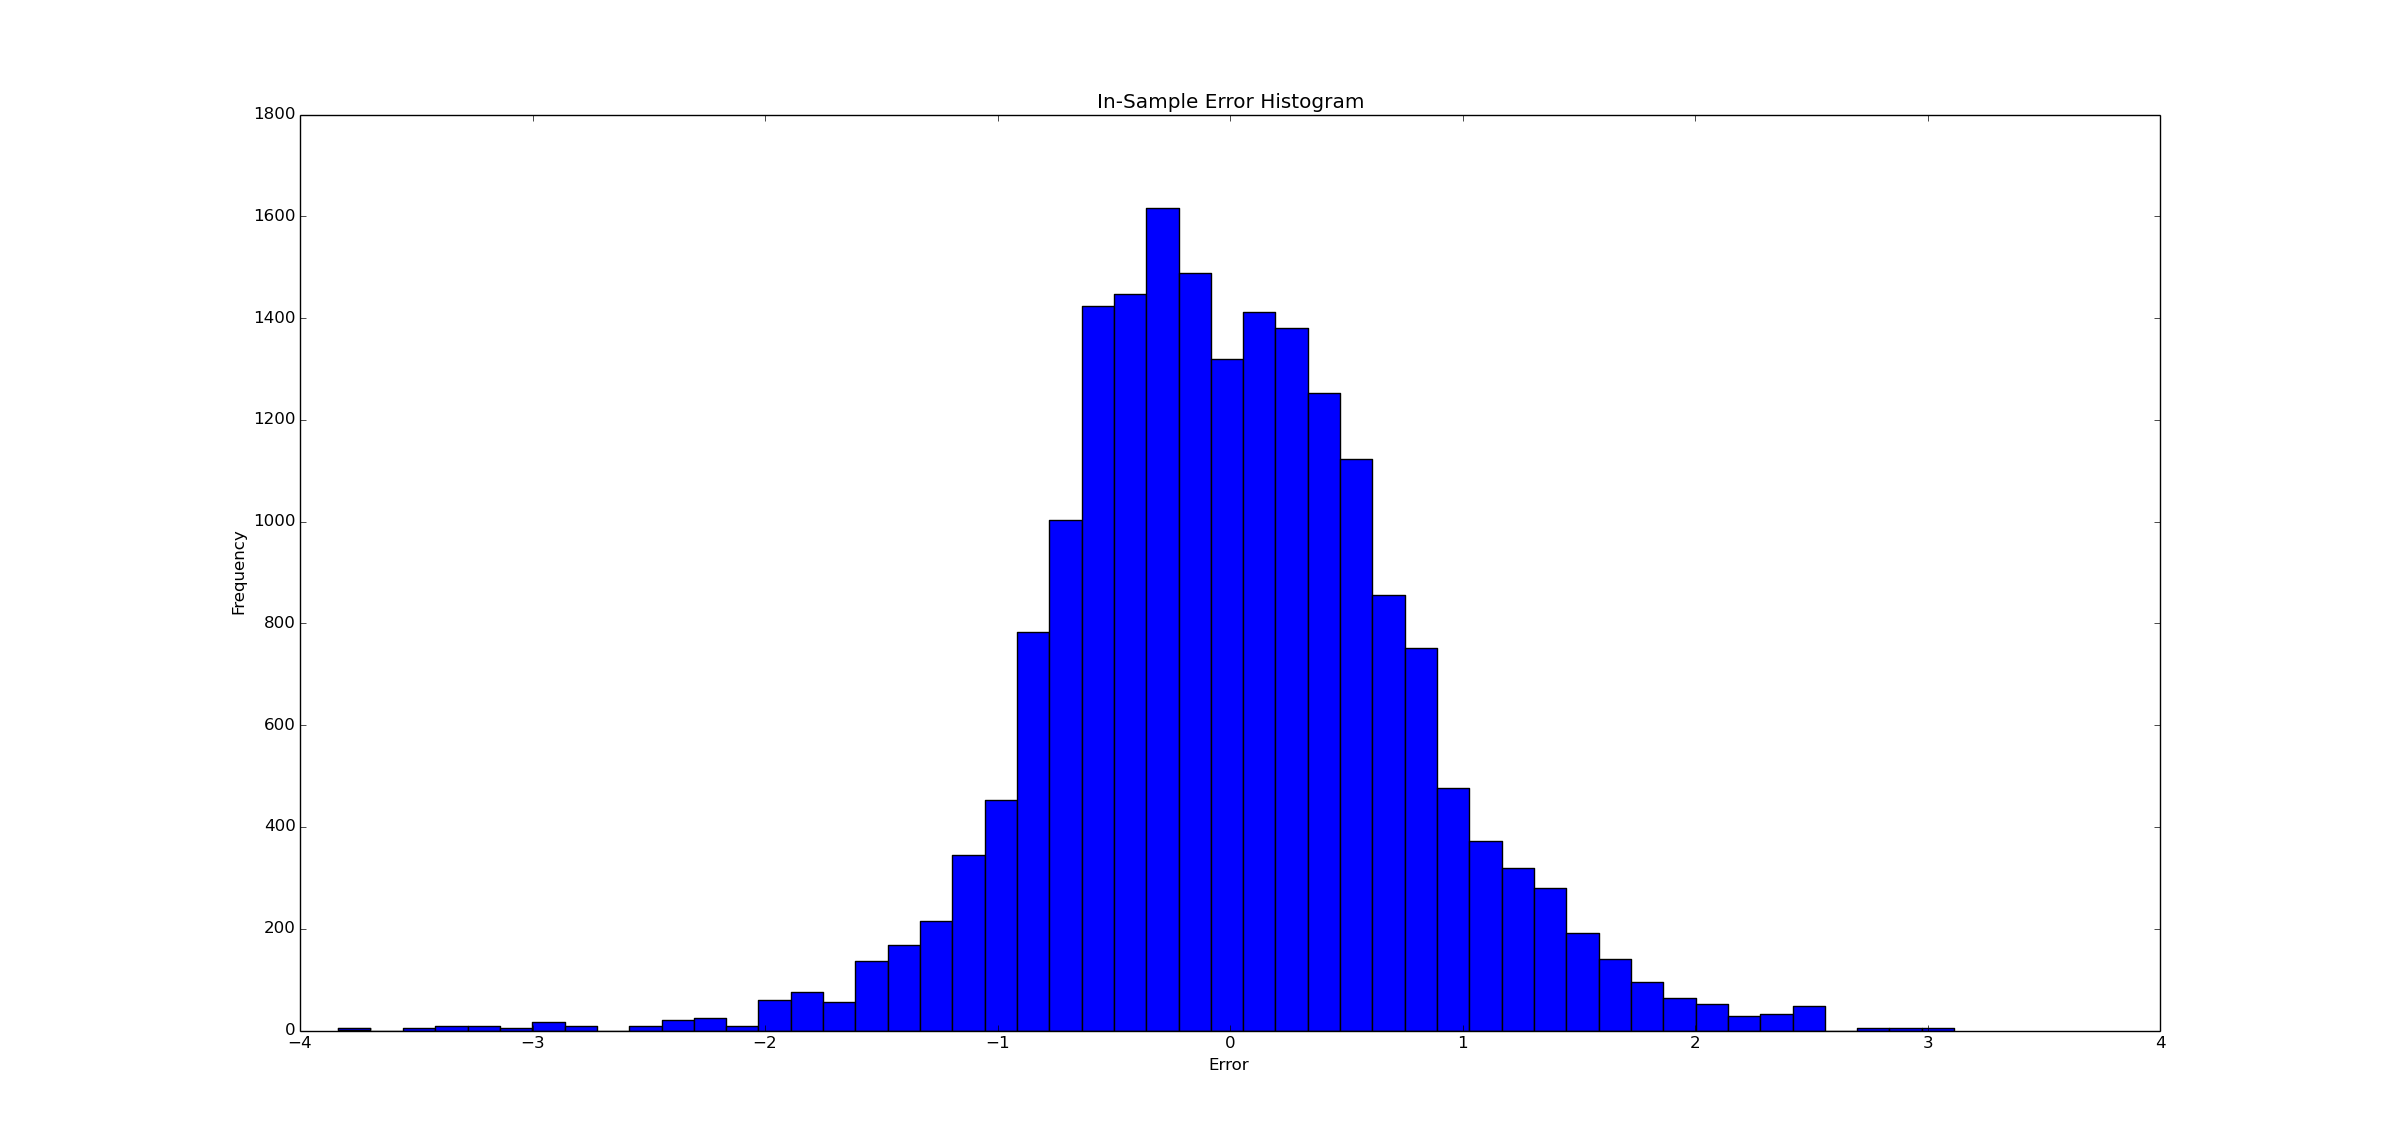
\includegraphics[width=1\textwidth]{figures/task1/is_error_histogram}
    \caption{In-sample error histogram plotted with matplotlib}
    \label{fig:is_task1}
\end{figure}

Figures \ref{fig:oos_task1} and \ref{fig:is_task1} show the out-of-sample and in-sample error histograms. They look similar, but Figure \ref{fig:is_task1} has higher frequencies, because the concatenated error vector has more elements.

\vspace{5mm} %5mm vertical space

The average error and variance for the out-of-sample and in-sample are reported in the following table:

\begin{center}
    \begin{tabular}{ | l | l | l |}
    \hline
     & \textbf{average error} & \textbf{variance}  \\ \hline
   	 \textbf{out-of-sample} & 9.83496755747e-13 & 0.563154062989 \\ \hline
   	 \textbf{in-sample} & 9.83614260773e-13 & 0.563154062989 \\ \hline
    \end{tabular}
\end{center}

\section{Task 2: Wine Quality Prediction with K Nearest Neighbors}

In the second task, scikit-learn's KNeighborRegressor method was used to predict wine quality with k nearest neighbors. Usage of method is similar to method used in the first task. The number of neighbors is passed as an argument. The method has optional arguments like algorithm and weights. The weights argument defaults to uniform weights. The API does not specify default algorithm, but I suppose auto is used and the method tries to decide the most appropriate algorithm based on the values passed to fit method. The following method was written to setup model to calculate k nearest neighbors for asked k=1..8:

\begin{lstlisting}[language=Python]
# Calculates model with K nearest neighbors, returns the model
def calculateKNearestNeighborsModel(data, numberOfNeighbors):
	# Select input variables as x and typecast to numpy array
	x = np.array(data.iloc[0:,0:11])
	# Select output variable (quality) as y and typecast to numpy array
	y = np.array(data.quality)
	neighbors = KNeighborsRegressor(n_neighbors=numberOfNeighbors)
	neighbors.fit(x, y)
	return neighbors
\end{lstlisting}

Now prediction can be done by passing a sample as argument for the "predict method". If k \textgreater 1, average of k nearest neighbors quality attribute is returned. Calculating out-of-sample and in-sample error vector was done similarly than in Task 1.

% In-sample k=1
\begin{figure}[H]
    \centering
    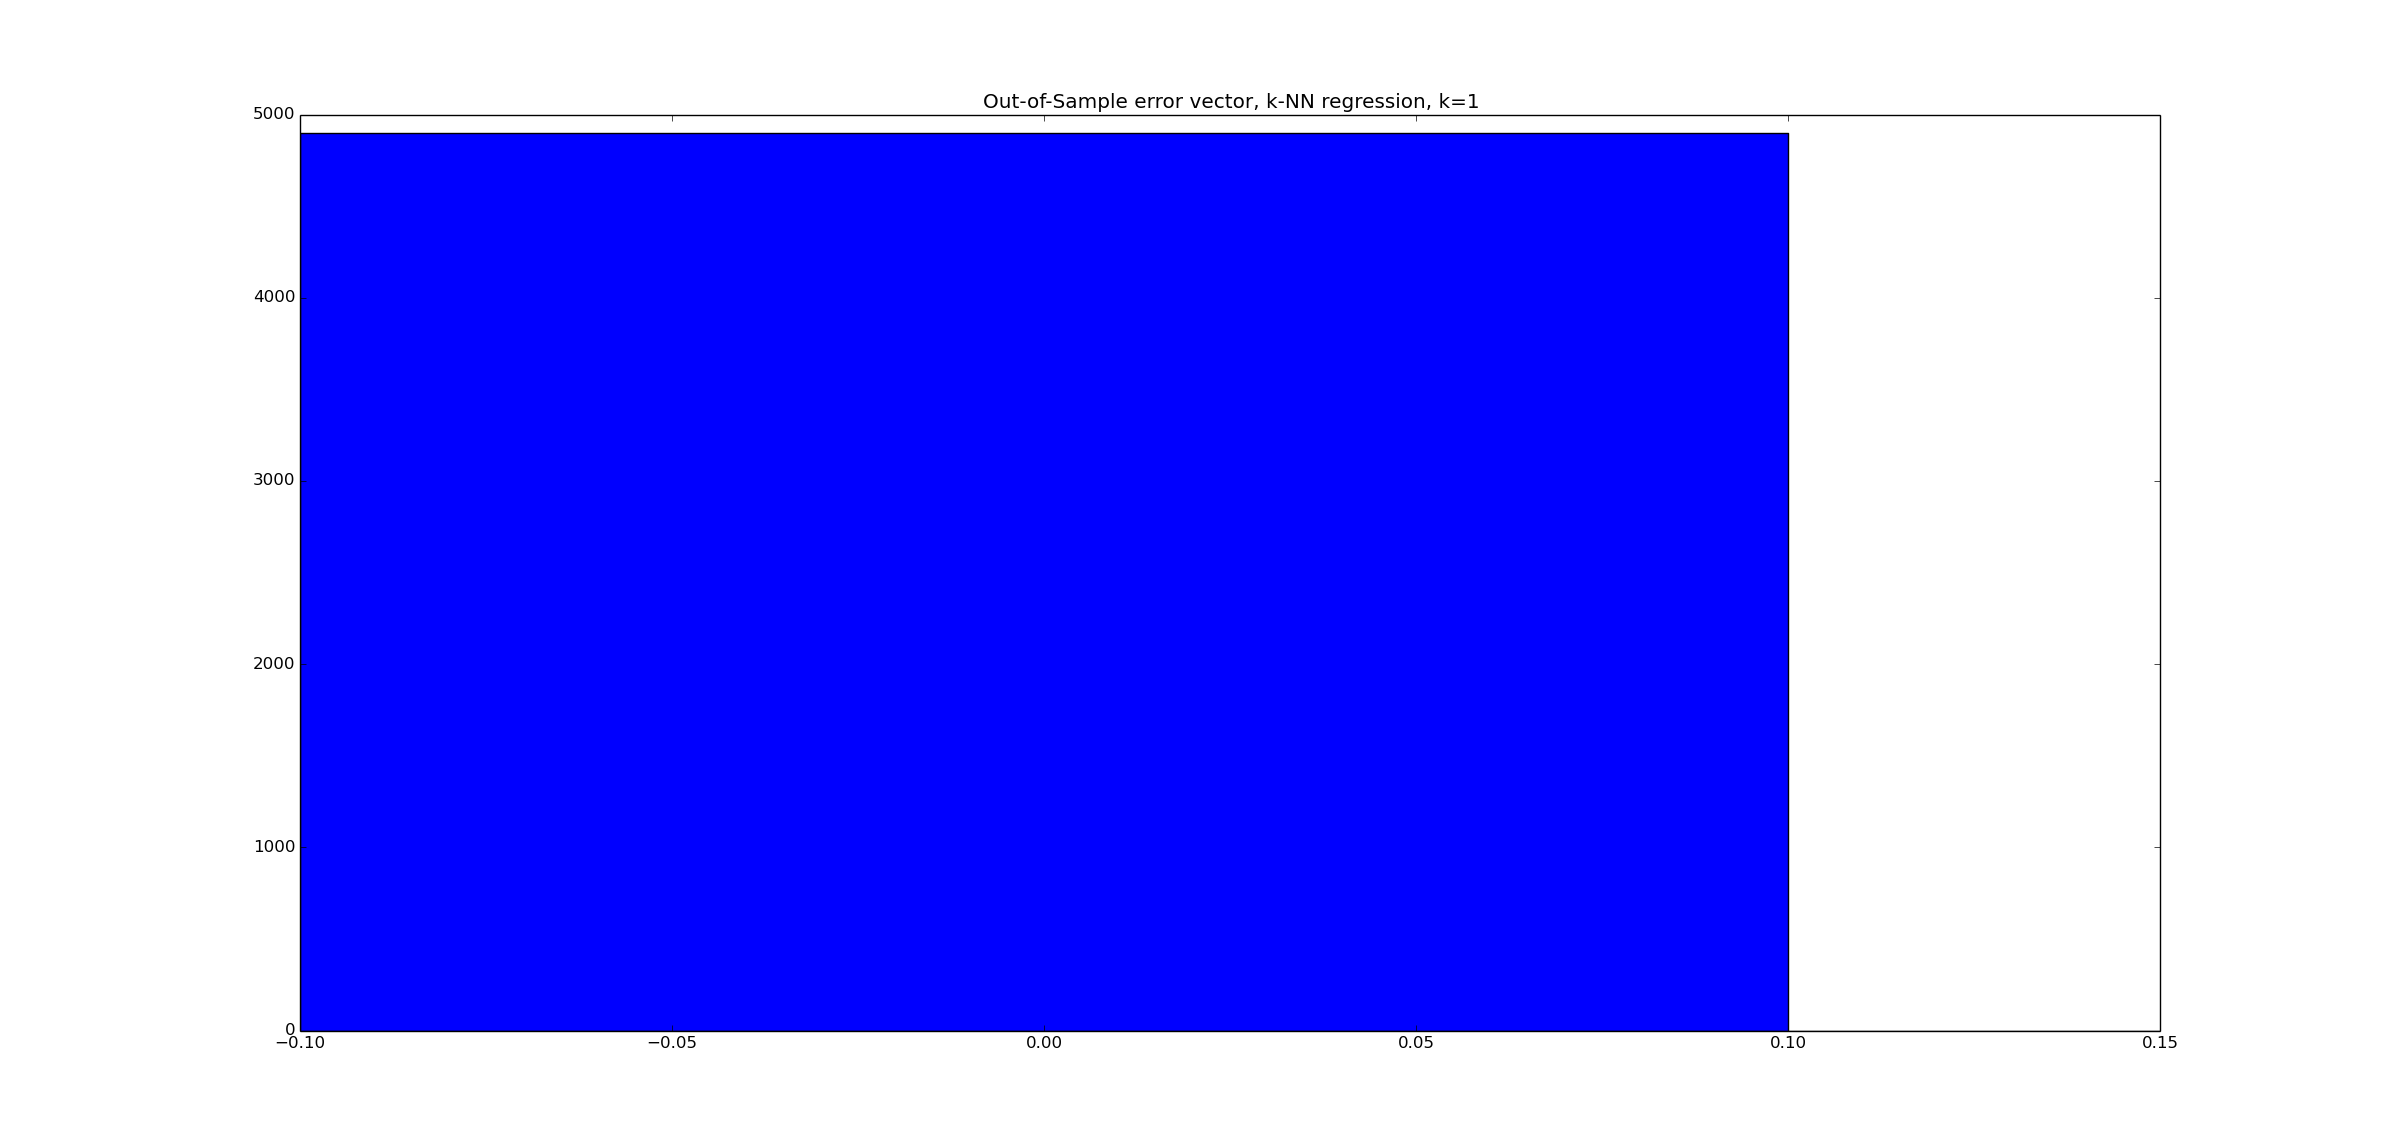
\includegraphics[width=1\textwidth]{figures/task2/k1_oos}
    \caption{Out-of-sample error histogram, k=1. Plotted with matplotlib}
    \label{fig:k1_oos_task2}
\end{figure}

Figure \ref{fig:k1_oos_task2} shows the out-of-sample histogram for k=1. It seems a bit weird. This happens, because the query set matches the training set. Hence, the nearest neighbor of each point is the point itself, at distance of zero. Therefore, the concatenated error vectors are full of zeros. The in-sample error histogram is similar with higher frequencies. The figure is omitted from this report. The data could have been split to two parts, so the training set and query set would have been different.

To decide k best, out-of-sample mean errors for k=1..8 were printed:

\begin{lstlisting}[language=Python]
Out-of-sample mean error when neighbors 1 : 0.0
Out-of-sample mean error when neighbors 2 : -0.0134748877093
Out-of-sample mean error when neighbors 3 : -0.0101401932762
Out-of-sample mean error when neighbors 4 : -0.0114842792977
Out-of-sample mean error when neighbors 5 : -0.0145773785218
Out-of-sample mean error when neighbors 6 : -0.0162991697291
Out-of-sample mean error when neighbors 7 : -0.0147290439246
Out-of-sample mean error when neighbors 8 : -0.014623315639
\end{lstlisting}

k=1 was excluded for the abovementioned reason. So, k best is k=3.

% Out-of-sample k=3
\begin{figure}[H]
    \centering
    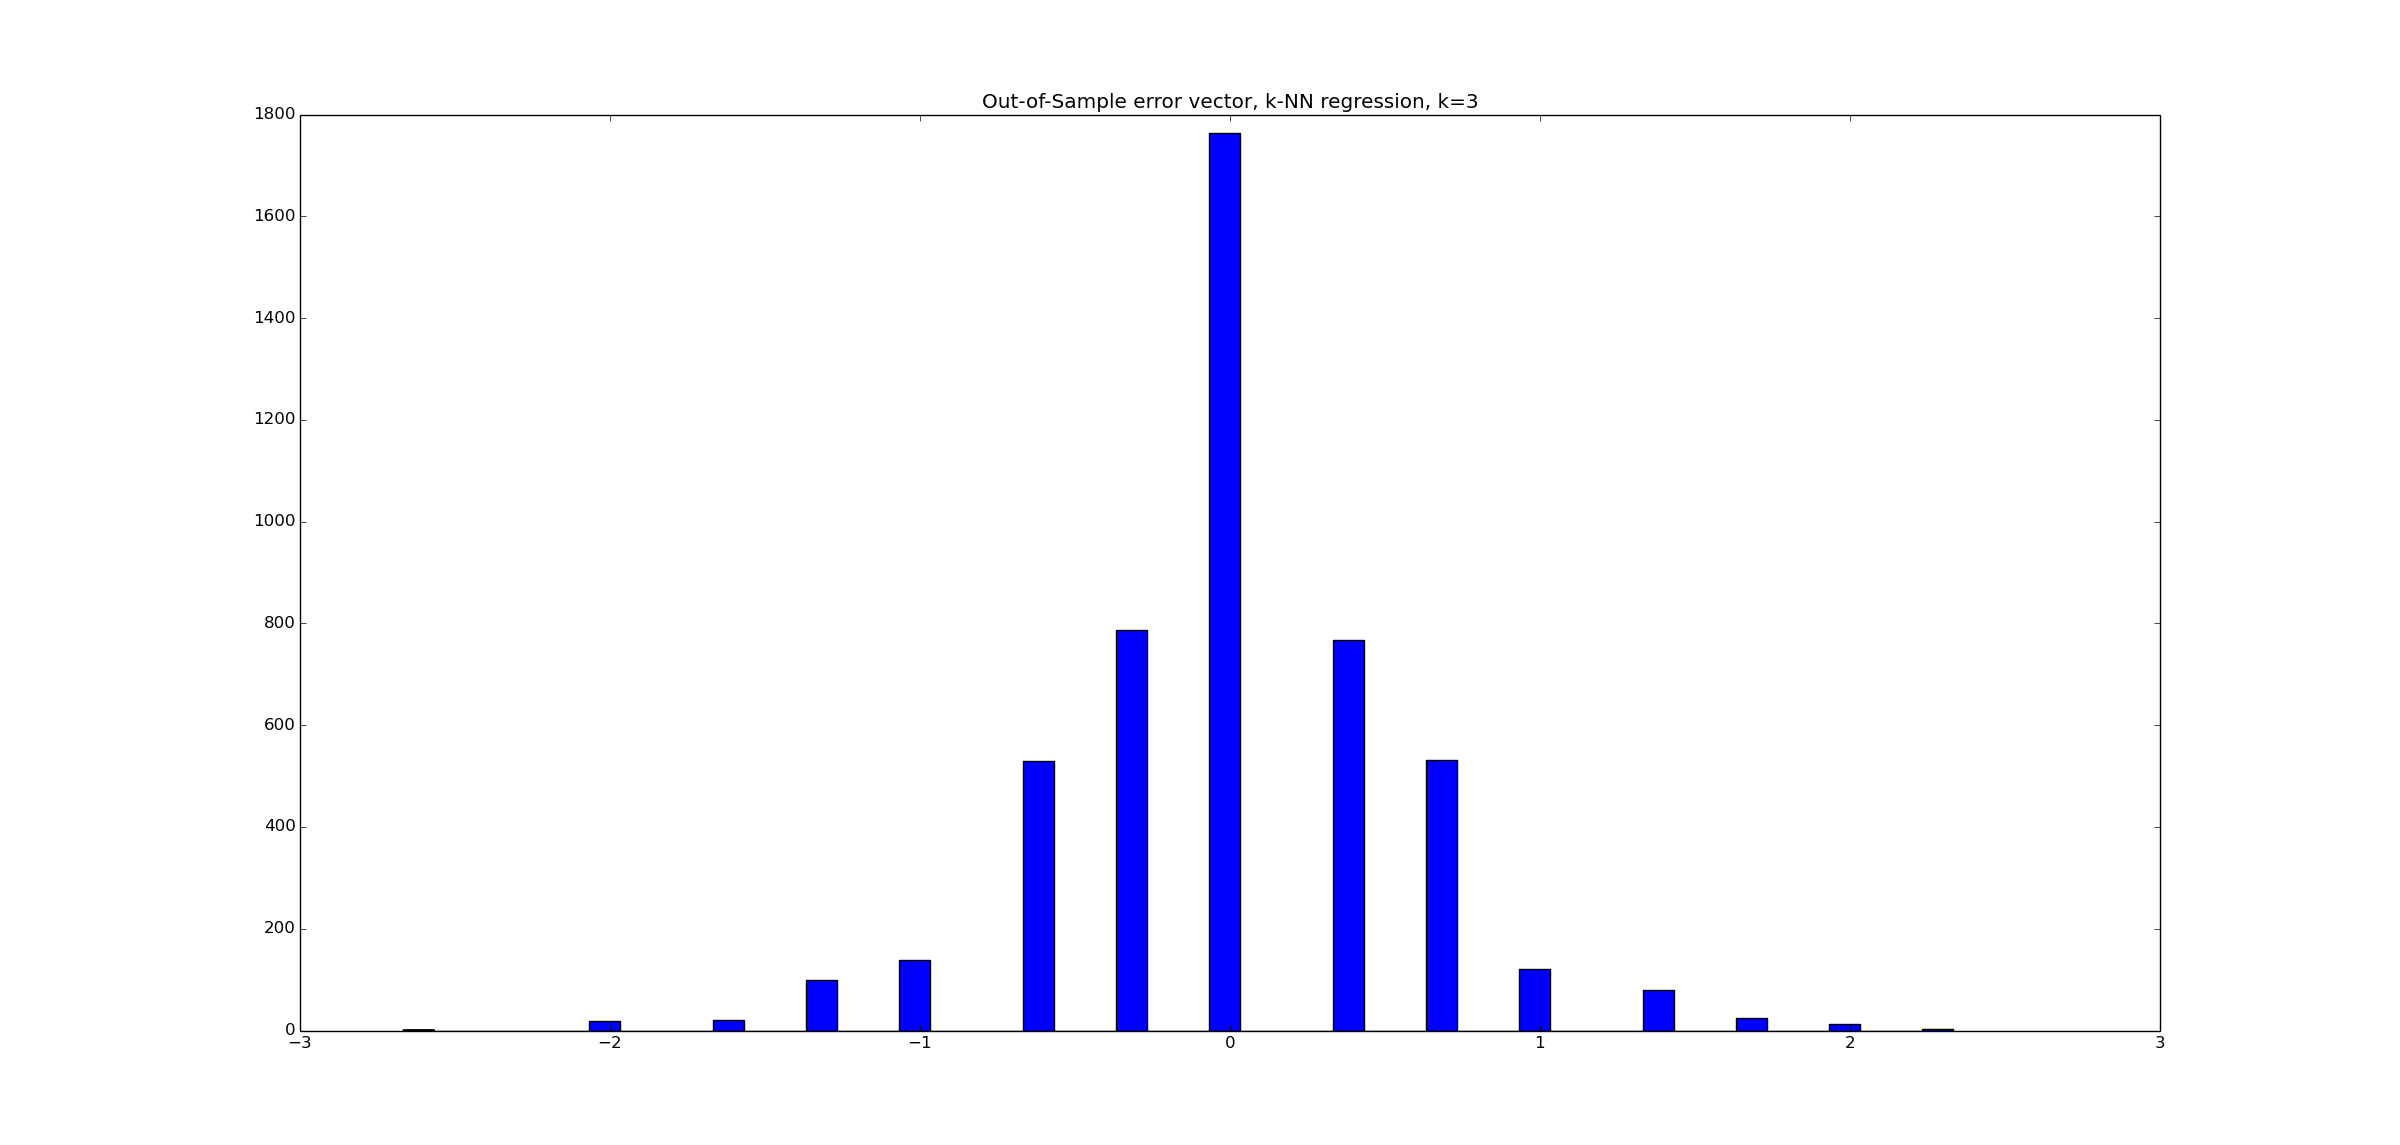
\includegraphics[width=1\textwidth]{figures/task2/k3_oos}
    \caption{Out-of-sample error histogram, k=3. Plotted with matplotlib}
    \label{fig:k3_oos_task2}
\end{figure}

% In-sample k=3
\begin{figure}[H]
    \centering
    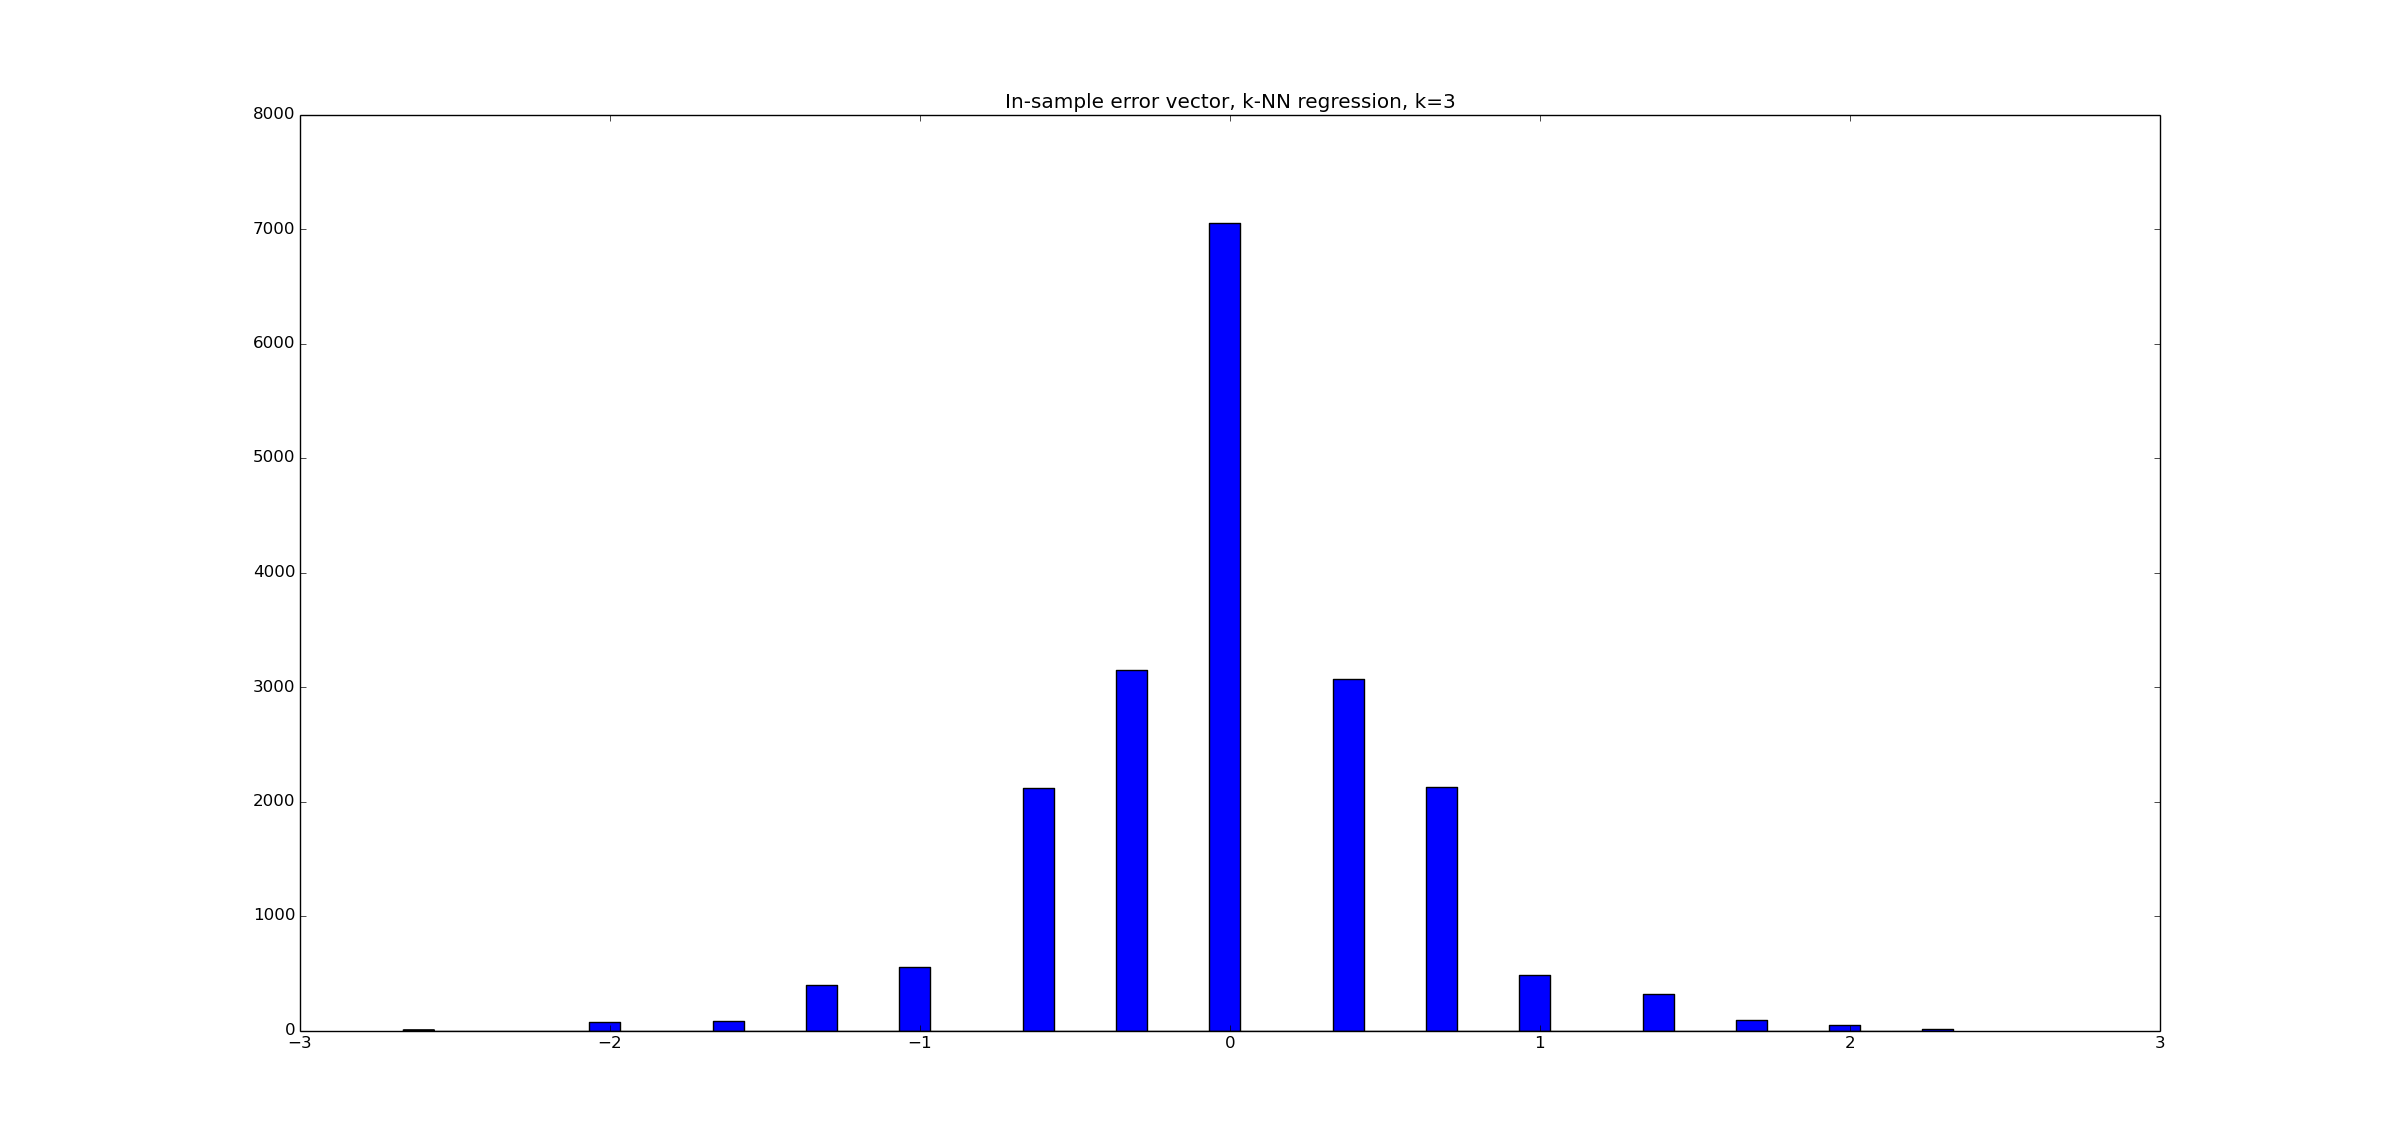
\includegraphics[width=1\textwidth]{figures/task2/k3_is}
    \caption{In-sample error histogram, k=3. Plotted with matplotlib}
    \label{fig:k3_is_task2}
\end{figure}

Figures \ref{fig:k3_oos_task2} and \ref{fig:k3_is_task2} show the error histograms for k=3. The histograms seem similar, but in-sample histogram has greater frequencies.

\vspace{5mm} %5mm vertical space

I also experimented a bit with scikit-learn NearestNeighbor method:

\begin{lstlisting}[language=Python]
x = np.array(data.iloc[0:,0:11])
y = np.array(data.quality)

nbrs = NearestNeighbors(n_neighbors=1, algorithm='ball_tree').fit(data)

distances, indices = nbrs.kneighbors(data)

for i in range(0, len(y)):
	print('Actual quality: ' + str(y[i]) + ' predicted quality: ' + str(y[indices[i][0]]))
	print(y[i] == y[indices[i][0]])
\end{lstlisting}

The method returns distances and indices of nearest neighbors for all data points. Index refers to the index in the training data. So, if k \textgreater 1 the average needs to be calculated for nearest neighbors to predict quality. Given this, it was easier to use KNeighborRegressor for this task.

\end{document}